% One editable, unified architecture figure. Build from the repository root:
%   mkdir -p figures/architecture
%   tectonic --outdir figures/architecture docs/architecture.tex
% Generated outputs remain untracked in figures/.
%
% Source contract: model.py::{Block,DeltaModel.forward_column,
% DeltaModel.forward_iterations,multipass,_jittered_fused_input,
% _feedback_entry,KVCache}; pkda.py; moe.py.
% The outer feedback loop advances token/pass coordinates and the loop
% re-entry advances the column index at one token. Neither is a same-column
% algebraic cycle. Dotted cutaway leaders are not data edges.
\documentclass[tikz,border=10pt]{standalone}
\usepackage[T1]{fontenc}
\usepackage{tgheros}
\usepackage{amsmath,amssymb}
\renewcommand{\familydefault}{\sfdefault}
\usetikzlibrary{arrows.meta,calc,positioning,backgrounds}

\definecolor{ink}{HTML}{253044}
\definecolor{muted}{HTML}{667184}
\definecolor{line}{HTML}{AAB2BE}
\definecolor{soft}{HTML}{F7F8FA}
\definecolor{pink}{HTML}{F4D1E0}
\definecolor{yellow}{HTML}{F7ECB1}
\definecolor{blue}{HTML}{D0DFF6}
\definecolor{teal}{HTML}{BCE6E0}
\definecolor{coral}{HTML}{F5CFB5}
\definecolor{gold}{HTML}{F5DC9F}
\definecolor{mint}{HTML}{D0E9C0}
\definecolor{purple}{HTML}{DDD0F4}
\definecolor{purpleink}{HTML}{7B4CB4}
\definecolor{greenink}{HTML}{67904C}
\definecolor{tealink}{HTML}{198D91}

\newcommand{\smalltext}{\fontsize{9}{11.5}\selectfont}
\newcommand{\tinytext}{\fontsize{7.8}{10}\selectfont}
\newcommand{\cell}[3]{%
  \node[cellbox] (#1) at (8.2,#2) {};
  \node[font=\bfseries\smalltext] at (8.2,#2+.88) {#3};
  \node[strip,gqaop] (#1gqa) at (8.2,#2+.08)
    {\textbf{NoPE-GGQA + MoE}};
  \node[strip,pkdaop] (#1pkda) at (8.2,#2-.65)
    {\textbf{PKDA + MoE}\qquad $\times 3$};
  \draw[flow,thin] (#1pkda.north) -- (#1gqa.south);
}

\begin{document}
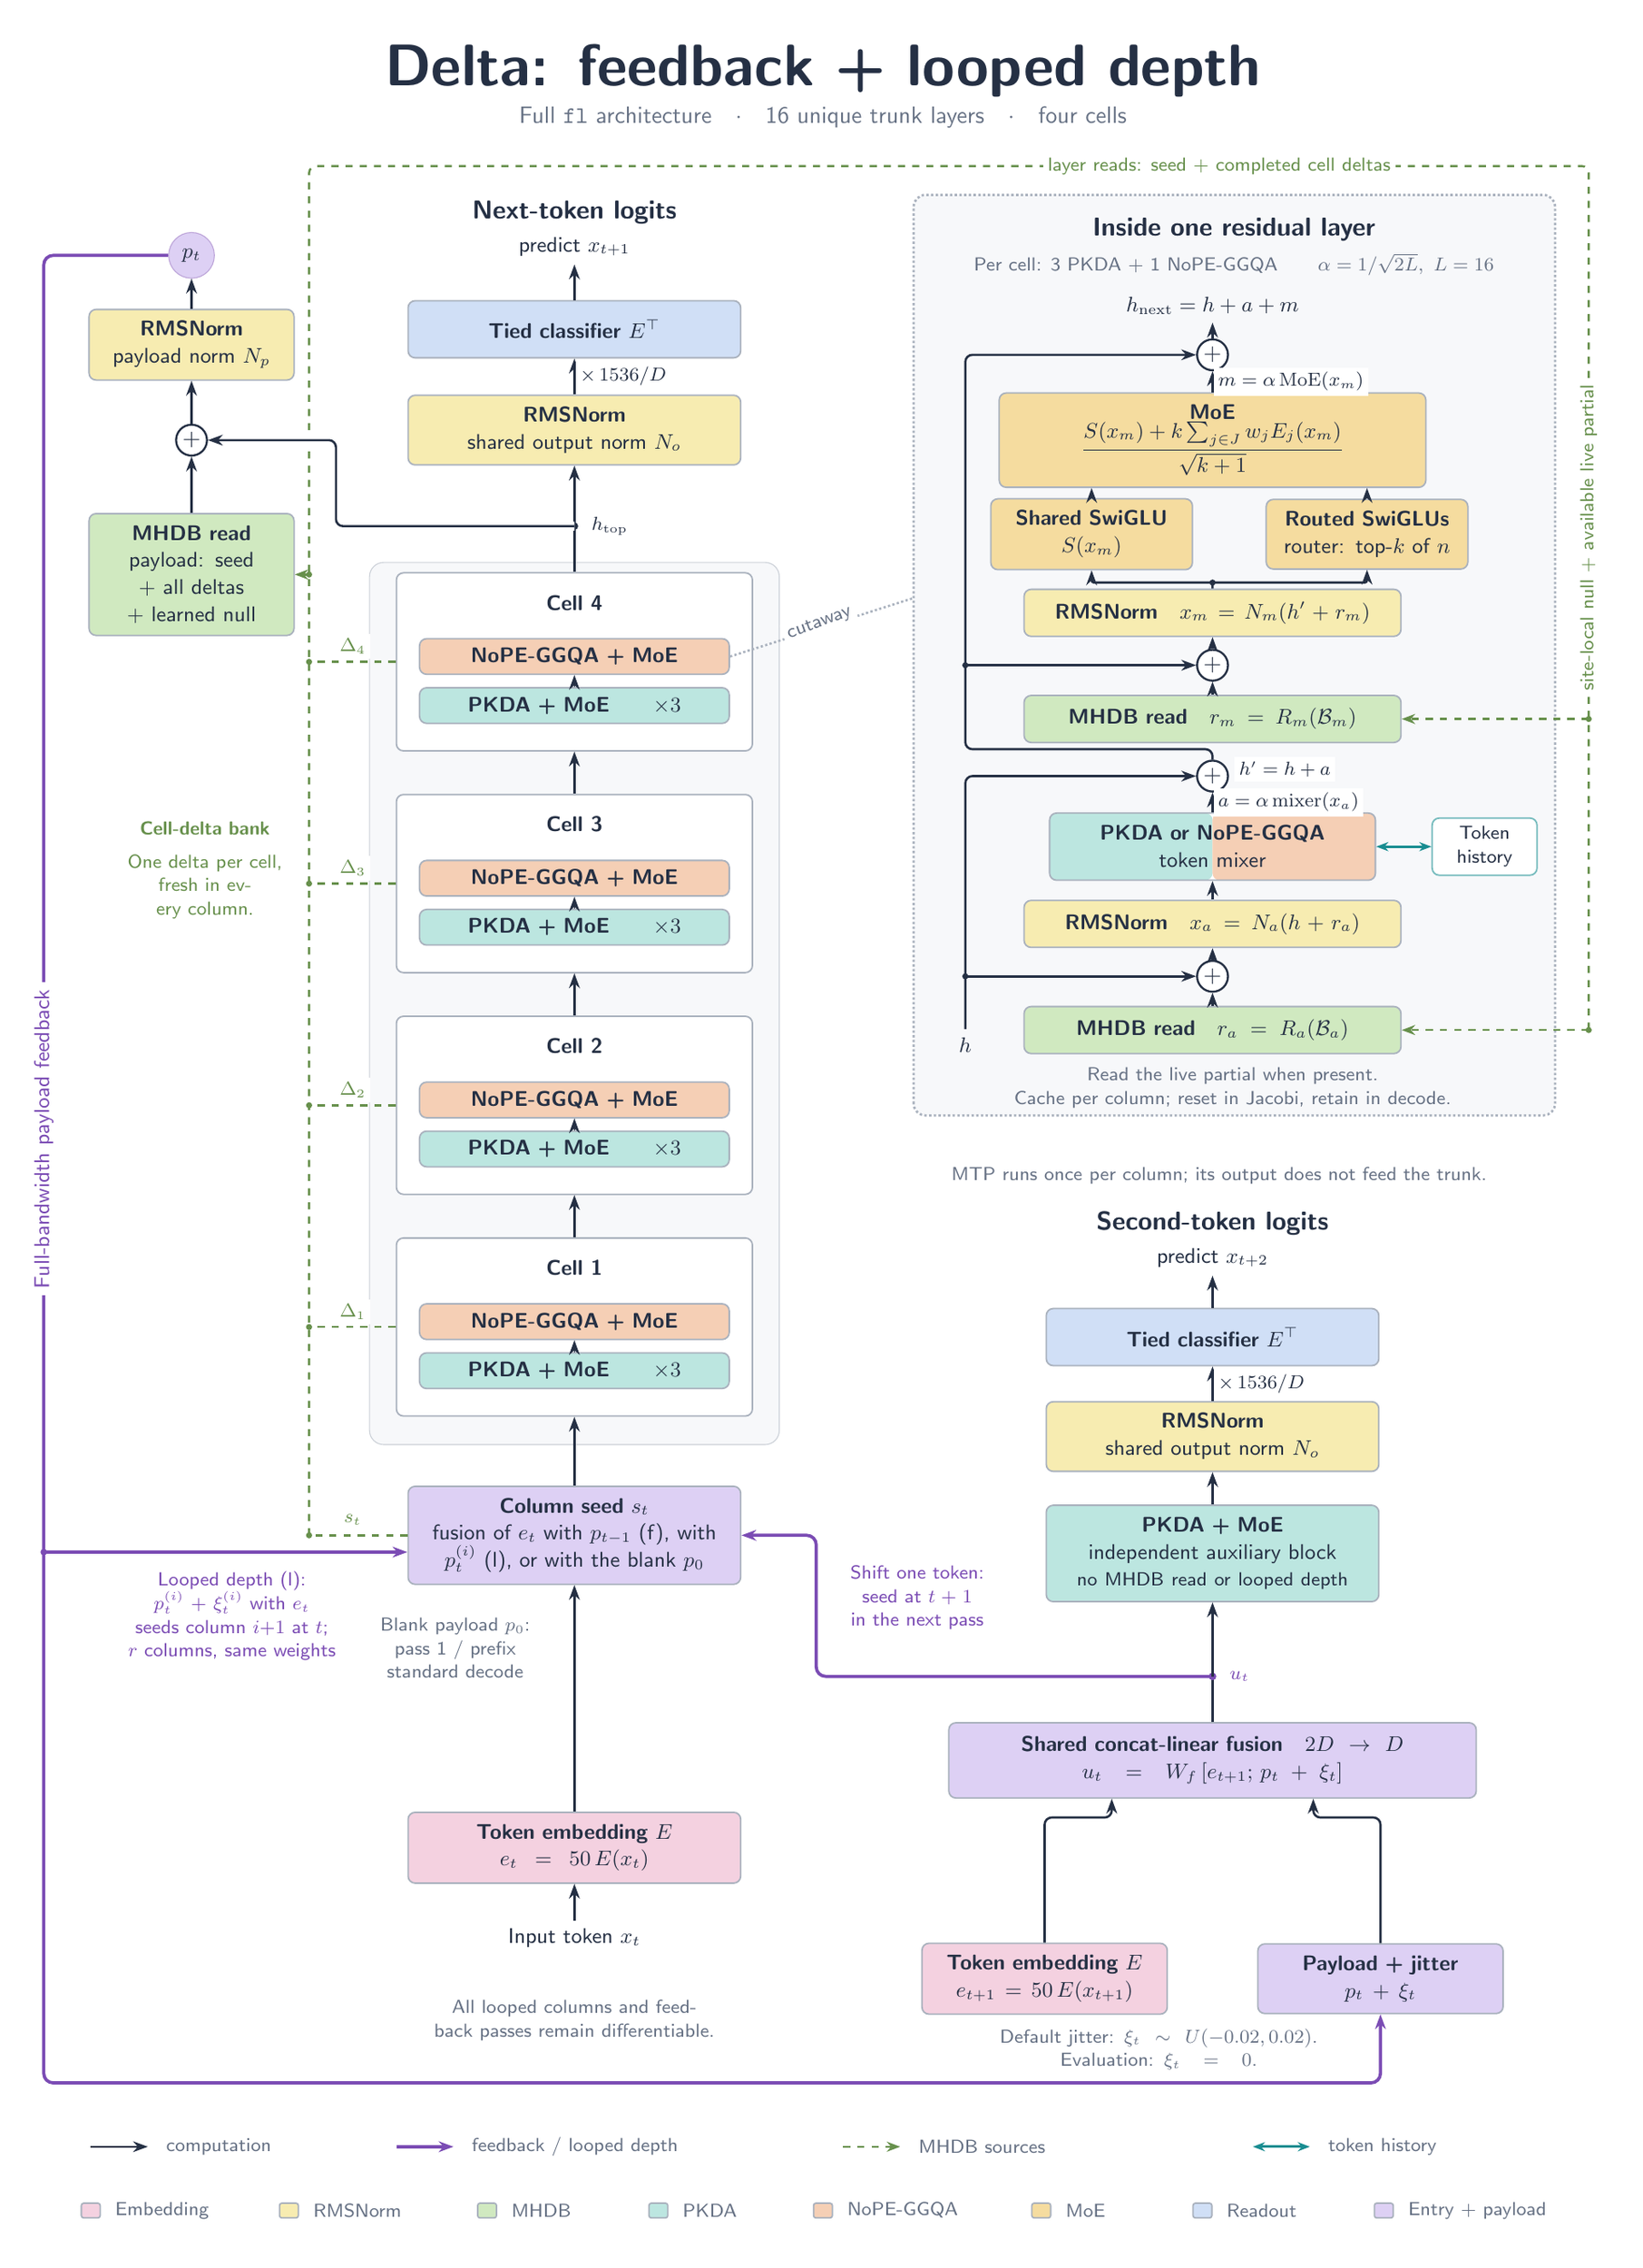
\begin{tikzpicture}[
  x=1cm,y=1cm,text=ink,font=\smalltext,
  box/.style={draw=line,fill=white,rounded corners=3pt,line width=.65pt,
    minimum height=.85cm,inner sep=5pt,align=center},
  % Semantic colors: use these styles for every occurrence of an operation.
  tokenop/.style={fill=pink},
  normop/.style={fill=yellow},
  mhdbop/.style={fill=mint},
  pkdaop/.style={fill=teal},
  gqaop/.style={fill=coral},
  moeop/.style={fill=gold},
  fusionop/.style={fill=purple},
  readoutop/.style={fill=blue},
  mixertype/.style={path picture={
    \fill[teal] (path picture bounding box.south west)
      rectangle (path picture bounding box.north);
    \fill[coral] (path picture bounding box.south)
      rectangle (path picture bounding box.north east);
  }},
  cellbox/.style={box,minimum width=5.3cm,minimum height=2.65cm},
  strip/.style={box,text width=4.4cm,minimum height=.53cm,
    inner sep=3pt,font=\smalltext},
  flow/.style={-{Stealth[length=2.2mm,width=1.6mm]},draw=ink,line width=.95pt},
  feedback/.style={flow,draw=purpleink,line width=1.35pt,rounded corners=4pt},
  bankwire/.style={draw=greenink,dashed,line width=.9pt},
  bankread/.style={bankwire,-{Stealth[length=2mm]}},
  state/.style={draw=tealink,line width=1pt,{Stealth[length=1.8mm]}-{Stealth[length=1.8mm]}},
  note/.style={text=muted,font=\tinytext,align=center},
  edgeword/.style={font=\tinytext,fill=white,inner sep=2pt},
  sum/.style={circle,draw=ink,fill=white,minimum size=.46cm,
    inner sep=0pt,font=\normalsize,line width=.85pt}
]
\path[use as bounding box] (0,-.85) rectangle (23.75,32.2);

\node[font=\bfseries\fontsize{23}{27}\selectfont] at (11.9,31.5)
  {Delta: feedback + looped depth};
\node[note,font=\fontsize{10}{13}\selectfont] at (11.9,30.8)
  {Full \texttt{fl} architecture\quad $\cdot$\quad 16 unique trunk layers\quad $\cdot$\quad four cells};

% The main column is the single bottom-to-top spine.
\draw[draw=line!60,fill=soft,rounded corners=6pt]
  (5.15,11.05) rectangle (11.25,24.18);
\cell{cellone}{12.8}{Cell 1}
\cell{celltwo}{16.1}{Cell 2}
\cell{cellthree}{19.4}{Cell 3}
\cell{cellfour}{22.7}{Cell 4}

\node[font=\smalltext] (tokens) at (8.2,3.7) {Input token $x_t$};
\node[box,tokenop,text width=4.6cm] (embedding) at (8.2,5.05)
  {\textbf{Token embedding $E$}\\$e_t=50\,E(x_t)$};
\node[box,fusionop,text width=4.6cm] (seed) at (8.2,9.7)
  {\textbf{Column seed $s_t$}\\fusion of $e_t$ with $p_{t-1}$ (f), with $p_t^{(i)}$ (l), or with the blank $p_0$};
\draw[flow] (tokens) -- (embedding);
\draw[flow] (embedding) -- (seed);
\node[note,anchor=east,text width=2.8cm] at (7.95,8.02)
  {Blank payload $p_0$:\\pass 1 / prefix\\standard decode};
\draw[flow] (seed) -- (cellone);
\draw[flow] (cellone) -- (celltwo);
\draw[flow] (celltwo) -- (cellthree);
\draw[flow] (cellthree) -- (cellfour);

\coordinate (top) at (8.2,24.72);
\node[box,normop,text width=4.6cm] (finalnorm) at (8.2,26.15)
  {\textbf{RMSNorm}\\shared output norm $N_o$};
\node[box,readoutop,text width=4.6cm] (classifier) at (8.2,27.65)
  {\textbf{Tied classifier $E^\top$}};
\node[align=center,font=\bfseries\fontsize{11}{14}\selectfont]
  (mainoutput) at (8.2,29.15) {Next-token logits\\\normalfont\smalltext predict $x_{t+1}$};
\draw[flow] (cellfour) -- (finalnorm);
\fill[ink] (top) circle (1.6pt);
\node[anchor=west,edgeword] at (8.38,24.72) {$h_{\mathrm{top}}$};
\draw[flow] (finalnorm) -- node[right,edgeword] {$\times\,1536/D$} (classifier);
\draw[flow] (classifier) -- (mainoutput);

% One accumulated delta per physical cell; the trunk and cutaway read only
% causally available contributions. Every MHDB site owns its own null.
\draw[bankwire,rounded corners=3pt] (4.25,9.7) -- (4.25,30.08)
  -- (23.3,30.08) -- (23.3,17.22);
\foreach \name/\y/\value in {seed/9.7/s_t,cellone/12.8/\Delta_1,celltwo/16.1/\Delta_2,cellthree/19.4/\Delta_3,cellfour/22.7/\Delta_4} {
  \draw[bankwire] (\name.west) -- (4.25,\y);
  \fill[greenink] (4.25,\y) circle (1.3pt);
  \node[edgeword,text=greenink] at (4.9,\y+.23) {$\value$};
}
\node[note,text width=2.5cm,text=greenink] at (2.7,19.6)
  {\textbf{Cell-delta bank}\\[4pt]
   One delta per cell,\\fresh in every column.};
\node[edgeword,text=greenink] at (17.8,30.08)
  {layer reads: seed + completed cell deltas};
\node[rotate=90,edgeword,text=greenink] at (23.3,24.55)
  {site-local null + available live partial};

% Payload write retains the direct top-state path, before final readout norm.
% Its learned RMSNorm writes the payload without an additional fixed scale.
\node[box,mhdbop,text width=2.7cm] (payloadroute) at (2.5,24.0)
  {\textbf{MHDB read}\\payload: seed + all deltas\\+ learned null};
\draw[bankread] (4.25,24.0) -- (payloadroute.east);
\fill[greenink] (4.25,24.0) circle (1.3pt);
\node[sum] (payloadadd) at (2.5,26.0) {$+$};
\draw[flow] (payloadroute) -- (payloadadd);
\draw[flow,rounded corners=3pt,preaction={draw=white,line width=3.8pt}]
  (top) -- (4.65,24.72) -- (4.65,26.0) -- (payloadadd.east);
\node[box,normop,text width=2.7cm] (payloadnorm) at (2.5,27.42)
  {\textbf{RMSNorm}\\payload norm $N_p$};
\node[circle,draw=purpleink!50,fusionop,minimum size=.68cm,inner sep=0pt]
  (payload) at (2.5,28.75) {$p_t$};
\draw[flow] (payloadadd) -- (payloadnorm);
\draw[flow] (payloadnorm) -- (payload);

% The outer feedback path carries p_t to fusion with e_{t+1}=50 E(x_{t+1}).
% Both token paths share E; one lookup serves the whole row.
% Fusion is computed once and reused by MTP and shifted feedback.
\node[box,fusionop,text width=3.3cm] (jitter) at (20.2,3.1)
  {\textbf{Payload + jitter}\\$p_t+\xi_t$};
\draw[feedback] (payload.west) -- (.3,28.75) -- (.3,1.55)
  -- (20.2,1.55) -- (jitter.south);
\node[rotate=90,text=purpleink,font=\smalltext,fill=white,inner sep=3pt]
  at (.3,15.6) {Full-bandwidth payload feedback};
% The loop re-entry: the same jittered payload, fused with this token's own
% embedding, seeds the next column at the same position.
\draw[feedback] (.3,9.45) -- (seed.west |- 0,9.45);
\fill[purpleink] (.3,9.45) circle (1.4pt);
\node[note,text=purpleink,text width=3.5cm,anchor=north] at (3.1,9.28)
  {Looped depth (l): $p_t^{(i)}+\xi_t^{(i)}$ with $e_t$\\
   seeds column $i{+}1$ at $t$;\\$r$ columns, same weights};
\node[box,tokenop,text width=3.3cm] (nextembedding) at (15.2,3.1)
  {\textbf{Token embedding $E$}\\$e_{t+1}=50\,E(x_{t+1})$};
\node[box,fusionop,text width=7.5cm,minimum height=1.12cm]
  (fusion) at (17.7,6.35)
  {\textbf{Shared concat-linear fusion}\quad $2D\to D$\\
   $u_t=W_f\,[e_{t+1};\,p_t+\xi_t]$};
\draw[flow,rounded corners=3pt] (nextembedding.north) -- (15.2,5.5)
  -| ($(fusion.south)+(-1.5,0)$);
\draw[flow,rounded corners=3pt] (jitter.north) -- (20.2,5.5)
  -| ($(fusion.south)+(1.5,0)$);
\coordinate (fused) at (17.7,7.6);
\draw[draw=ink,line width=.95pt] (fusion.north) -- (fused);
\fill[purpleink] (fused) circle (1.6pt);
\node[edgeword,anchor=west,text=purpleink] at (17.88,7.6) {$u_t$};
\draw[feedback] (fused) -- (11.8,7.6) -- (11.8,9.7) -- (seed.east);
\node[note,text=purpleink,text width=2.3cm,anchor=west] at (12.03,8.77)
  {Shift one token:\\seed at $t+1$\\in the next pass};
\node[note,text width=6.6cm] at (16.9,2.05)
  {Default jitter: $\xi_t\sim U(-0.02,0.02)$.\\Evaluation: $\xi_t=0$.};

% MTP is a connected side branch of the very same fusion tensor.
\node[box,pkdaop,text width=4.6cm,minimum height=1.2cm]
  (mtp) at (17.7,9.43)
  {\textbf{PKDA + MoE}\\independent auxiliary block\\\tinytext no MHDB read or looped depth};
\draw[flow] (fused) -- (mtp.south);
\node[box,normop,text width=4.6cm] (mtpnorm) at (17.7,11.17)
  {\textbf{RMSNorm}\\shared output norm $N_o$};
\node[box,readoutop,text width=4.6cm] (mtpclassifier) at (17.7,12.65)
  {\textbf{Tied classifier $E^\top$}};
\node[align=center,font=\bfseries\fontsize{11}{14}\selectfont]
  (mtpoutput) at (17.7,14.1)
  {Second-token logits\\\normalfont\smalltext predict $x_{t+2}$};
\draw[flow] (mtp) -- (mtpnorm);
\draw[flow] (mtpnorm) -- node[right,edgeword] {$\times\,1536/D$} (mtpclassifier);
\draw[flow] (mtpclassifier) -- (mtpoutput);
\node[note,text width=8.2cm] at (17.8,15.05)
  {MTP runs once per column; its output does not feed the trunk.};

% One attached cutaway, not a second architecture or a separate panel.
\draw[draw=line,densely dotted,line width=1pt,fill=soft,rounded corners=5pt]
  (13.25,15.95) rectangle (22.8,29.65);
\draw[draw=line,densely dotted,line width=.95pt]
  (cellfourgqa.east) -- (13.25,23.65);
\node[edgeword,rotate=20,text=muted] at (11.85,23.27) {cutaway};
\node[font=\bfseries\fontsize{11}{14}\selectfont] at (18.02,29.13)
  {Inside one residual layer};
\node[note] at (18.02,28.61)
  {Per cell: 3 PKDA + 1 NoPE-GGQA\qquad $\alpha=1/\sqrt{2L},\ L=16$};
\node (layerout) at (17.7,28.0) {$h_{\mathrm{next}}=h+a+m$};
\node[sum] (addm) at (17.7,27.27) {$+$};
\node[box,moeop,text width=6.0cm,minimum height=.9cm]
  (mixexperts) at (17.7,26.0)
  {\textbf{MoE}\\$\displaystyle
    \frac{S(x_m)+k\sum_{j\in J}w_jE_j(x_m)}{\sqrt{k+1}}$};
\node[box,moeop,text width=2.65cm,minimum height=1.0cm]
  (sharedexpert) at (15.9,24.6)
  {\textbf{Shared SwiGLU}\\$S(x_m)$};
\node[box,moeop,text width=2.65cm,minimum height=1.0cm]
  (routedexperts) at (20.0,24.6)
  {\textbf{Routed SwiGLUs}\\router: top-$k$ of $n$};

% Every branch has the same explicit read -> add -> norm structure as the
% payload writer. A learned MHDB query reads the bank, not the live residual;
% h or h' joins that read at + and also follows its untouched residual bypass.
\node[box,normop,text width=5.4cm,minimum height=.7cm,inner sep=3pt]
  (normm) at (17.7,23.43)
  {\textbf{RMSNorm}\quad $x_m=N_m(h'+r_m)$};
\node[sum] (readaddm) at (17.7,22.65) {$+$};
\node[box,mhdbop,text width=5.4cm,minimum height=.7cm,inner sep=3pt]
  (readm) at (17.7,21.85)
  {\textbf{MHDB read}\quad $r_m=R_m(\mathcal B_m)$};
\node[sum] (adda) at (17.7,21.0) {$+$};
\node[box,mixertype,text width=4.5cm,minimum height=1.0cm]
  (tokenmixer) at (17.7,19.95)
  {\textbf{PKDA or NoPE-GGQA}\\token mixer};
\node[box,normop,text width=5.4cm,minimum height=.7cm,inner sep=3pt]
  (norma) at (17.7,18.8)
  {\textbf{RMSNorm}\quad $x_a=N_a(h+r_a)$};
\node[sum] (readadda) at (17.7,18.02) {$+$};
\node[box,mhdbop,text width=5.4cm,minimum height=.7cm,inner sep=3pt]
  (reada) at (17.7,17.22)
  {\textbf{MHDB read}\quad $r_a=R_a(\mathcal B_a)$};
\node (layerin) at (14.02,17.0) {$h$};

\draw[flow] (reada) -- (readadda);
\draw[flow] (readadda) -- (norma);
\draw[flow] (norma) -- (tokenmixer);
\draw[flow] (tokenmixer) -- node[right,edgeword]
  {$a=\alpha\,\mathrm{mixer}(x_a)$} (adda);
\draw[flow] (readm) -- (readaddm);
\draw[flow] (readaddm) -- (normm);
\draw[flow,rounded corners=1pt] (normm.north) -- (17.7,23.88)
  -- (15.9,23.88) -- (sharedexpert.south);
\draw[flow,rounded corners=1pt] (17.7,23.88) -- (20.0,23.88)
  -- (routedexperts.south);
\fill[ink] (17.7,23.88) circle (1.3pt);
\draw[flow] (sharedexpert.north) -- (mixexperts.south -| sharedexpert.north);
\draw[flow] (routedexperts.north) -- (mixexperts.south -| routedexperts.north);
\draw[flow] (mixexperts) -- node[right,edgeword]
  {$m=\alpha\,\mathrm{MoE}(x_m)$} (addm);
\draw[flow] (addm) -- (layerout);

% The lower and upper residual rails each feed both their pre-norm sum and
% their post-sublayer sum. They never pass through the MHDB read itself.
\draw[flow,rounded corners=3pt] (layerin.north) -- (14.02,21.0) -- (adda.west);
\draw[flow] (14.02,18.02) -- (readadda.west);
\fill[ink] (14.02,18.02) circle (1.3pt);
\draw[flow,rounded corners=3pt] (adda.north) -- (17.7,21.4)
  -- (14.02,21.4) |- (addm.west);
\draw[flow] (14.02,22.65) -- (readaddm.west);
\fill[ink] (14.02,22.65) circle (1.3pt);
\node[edgeword,anchor=west] at (18.02,21.1) {$h'=h+a$};
\draw[bankread] (23.3,17.22) -- (reada.east);
\fill[greenink] (23.3,17.22) circle (1.3pt);
\draw[bankread] (23.3,21.85) -- (readm.east);
\fill[greenink] (23.3,21.85) circle (1.3pt);
\node[box,fill=white,draw=tealink!60,text width=1.35cm,font=\tinytext,inner sep=3pt]
  (history) at (21.75,19.95) {Token\\history};
\draw[state] (tokenmixer.east) -- (history.west);
\node[note,text width=8.8cm] at (18.0,16.36)
  {Read the live partial when present.\\
   Cache per column; reset in Jacobi, retain in decode.};

% Small labels stay adjacent to their mechanisms rather than becoming panels.
\node[note,text width=4.8cm] at (8.2,2.48)
  {All looped columns and feedback passes remain differentiable.};
\draw[flow] (1.0,.6) -- (1.85,.6);
\node[anchor=west,note] at (2.0,.6) {computation};
\draw[feedback] (5.55,.6) -- (6.4,.6);
\node[anchor=west,note] at (6.55,.6) {feedback / looped depth};
\draw[bankread] (12.2,.6) -- (13.05,.6);
\node[anchor=west,note] at (13.2,.6) {MHDB sources};
\draw[state] (18.3,.6) -- (19.15,.6);
\node[anchor=west,note] at (19.3,.6) {token history};
% Color and wire legends use the same styles as the diagram.
\foreach \x/\kind/\label in {
  1.0/tokenop/Embedding,3.95/normop/RMSNorm,6.9/mhdbop/MHDB,
  9.45/pkdaop/PKDA,11.9/gqaop/NoPE-GGQA,15.15/moeop/MoE,
  17.55/readoutop/Readout,20.25/fusionop/Entry + payload} {
  \node[box,\kind,minimum width=.28cm,minimum height=.22cm,
    inner sep=0pt,rounded corners=1pt] at (\x,-.35) {};
  \node[note,anchor=west] at (\x+.24,-.35) {\label};
}
\end{tikzpicture}
\end{document}
